\addcontentsline{toc}{chapter}{Messdaten} 
\label{Protokoll}

% \thispagestyle{empty}

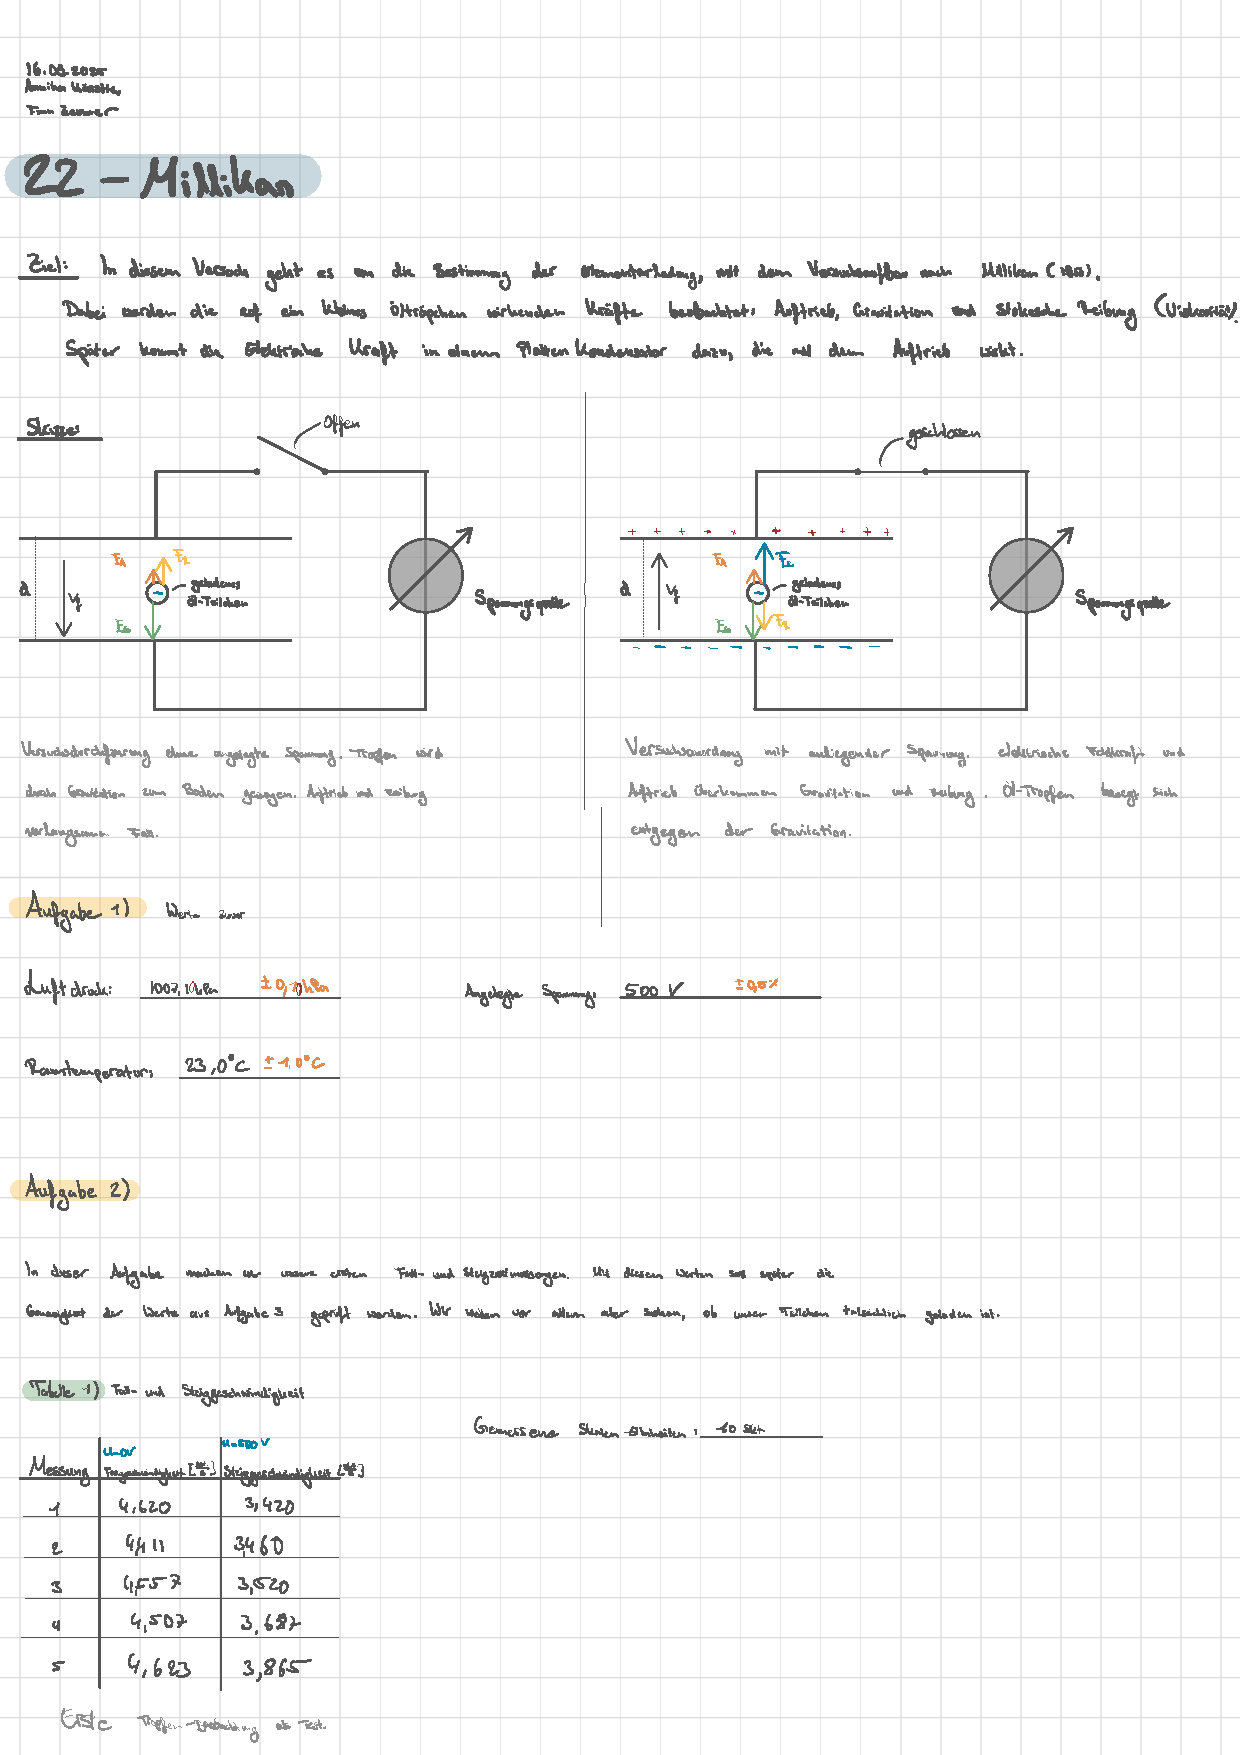
\includepdf[
  pages=1-3,               
  pagecommand={\thispagestyle{empty}} 
]{Protokolle/\versuchsnummer/Chapter/Messprotokoll.pdf}

\addcontentsline{lot}{table}{\protect\numberline{\thechapter.1} Pendellänge}
\addcontentsline{lot}{table}{\protect\numberline{\thechapter.2} (Vorläufige) Schwingdauer}
\addcontentsline{lot}{table}{\protect\numberline{\thechapter.3} GEnaue Bestimmung der Periodendauer}
\addcontentsline{lot}{table}{\protect\numberline{\thechapter.4} Bestimmung der Dämpfung}
